% Springer Nature template v12. Machine Vision and Applications requests iicol.
\documentclass[iicol,pdflatex,sn-mathphys-num]{sn-jnl}

\usepackage{graphicx}
\usepackage{booktabs}
\usepackage{multirow}
\usepackage{amsmath,amssymb,amsfonts}
\usepackage{amsthm}
\usepackage{xcolor}
\usepackage{array}

\hypersetup{
  pdftitle={Geometry-Defined Single-Owner PPE Evidence Allocation},
  pdfauthor={Yuge Lu, Sheng Huang, Qiuzu Lan, Yong Cai},
  pdfsubject={Geometry-defined PPE evidence allocation with a blinded adjudicated human ownership audit},
  pdfkeywords={personal protective equipment, evidence allocation, cross-worker contamination, selective decisions, geometry-defined representation}
}

\newtheorem{proposition}{Proposition}

\raggedbottom

\begin{document}

\title[Geometry-Defined Single-Owner PPE Evidence Allocation]{Geometry-Defined Single-Owner PPE Evidence Allocation and Cross-Worker Contamination Analysis}

\author*[1]{\fnm{Yuge} \sur{Lu}}\email{450671132@qq.com}
\author[1]{\fnm{Sheng} \sur{Huang}}
\author[1]{\fnm{Qiuzu} \sur{Lan}}
\author[1]{\fnm{Yong} \sur{Cai}}
\affil*[1]{\orgname{Guangxi Road And Bridge Engineering Group Co., Ltd.},
  \orgaddress{\city{Nanning}, \country{China}}}

\abstract{Personal protective equipment (PPE) monitoring is commonly evaluated as object detection, although an operational representation must prevent one worker's evidence from being copied to another worker and should allow uncertain cases to be reviewed. We study the Worker-Centric Selective Safety State Inference (RC-WSSI) protocol as deterministic single-owner helmet and vest evidence allocation followed by safe, unsafe, or review states. Four filename-group-disjoint roles separate detector training, detector validation, threshold selection, and final testing across five seeds, three folds, and two non-nested detector-training label budgets. The fixed high-to-low Clopper--Pearson sequence is reported only as a model-conditional feasibility diagnostic under an idealized independent worker-level Bernoulli model; infeasible selection returns review-all. At 10\% labels, the primary YOLOv8s pipeline obtains unsafe F1 $0.727$, cell-mean automatic-safe rate $0.112$, and cell-mean composite miss-or-safe rate $0.172$. Person-weighted and filename-group-macro composite rates are $0.184$ and $0.243$, with an observed worst filename-group/fold value of $0.486$. A revision-added post hoc sensitivity that treats reference-review workers as unsafe during selection and scoring gives automatic-safe/composite rates of $0.151/0.305$. At $\alpha=0.05$, only 2/15 and 5/15 cells retain a threshold at 5\% and 10\% labels. A blinded, independently adjudicated audit on 60 selected difficult images gives initial agreement of 587/597 assignments and RC-WSSI exact owner-set accuracy of $0.975$. A complementary source-stratified random audit uses 66 images and 334 PPE boxes with three open-candidate blind passes; 13 rows are ambiguous, and RC-WSSI matches 320/321 determinate human owner labels ($0.997$), while the original geometric candidate set contains 320/321 human owners. Global pooling matches 31/321 rows and creates 1,034 extra owner links on this random audit. These results support a single-owner representation and cross-worker-contamination analysis on sampled audits, not universal association superiority, a cluster-valid statistical guarantee, or deployment safety.}

\keywords{personal protective equipment, evidence allocation, cross-worker contamination, selective decisions, low-light vision, geometry-defined representation}

\maketitle

\section{Introduction}\label{sec:introduction}

Low-light tunnel construction combines small protective equipment, uneven illumination, occlusion, and crowded worker layouts. Recent detectors improve personal protective equipment (PPE) recognition under these conditions through low-light enhancement and detector redesign \cite{wang2023lowlight,malaikrisanachalee2025espcn,wu2025enhanced}. Few-shot construction-site recognition also reduces annotation demand \cite{wang2024fewshot}. These advances remain primarily object-centric: they report whether helmet, vest, or violation boxes were detected. A monitoring system, however, must decide whether a particular worker is safe, unsafe, or too uncertain for automatic action.

This distinction matters when multiple workers appear in one image. Pooling all PPE detections at image level can attach one worker's helmet or vest to another worker. It can therefore turn an unsafe worker into an apparently safe one. A fixed confidence threshold has a second limitation: it provides no explicit statement about the probability of this unsafe-to-safe decision. Conventional detector calibration improves confidence fidelity \cite{oksuz2023selfaware,pathiraja2023multiclass,le2018uncertainty}, but calibrated confidence alone does not specify which operational error is controlled or when the system must abstain.

We formulate PPE monitoring as a geometry-defined evidence-allocation representation with selective decisions. RC-WSSI first assigns PPE and violation evidence to the detected person with greatest geometric support. It then maps each matched person to \emph{safe}, \emph{unsafe}, or \emph{review}. The threshold-selection procedure applies a model-conditional diagnostic to the all-reference automatic-safe event, while matched unsafe-to-safe and end-to-end miss-or-safe quantities are reported as separate diagnostics. A held-out threshold-selection set chooses the most permissive threshold that passes the stated diagnostic. If the available unsafe reference persons cannot support that calculation, the method returns review-all instead of an automatic policy.

The threshold family has a useful structure: increasing the evidence threshold cannot create a new automatic-safe person. We use this nested safe set to implement a high-to-low fixed-sequence Clopper--Pearson (CP) diagnostic \cite{clopper1934confidence}. In this monotone setting, the sequence retains the same prefix as a full-grid ordinary Clopper--Pearson scan; its value is transparent feasibility reporting, not an empirical power advantage. This connects selective prediction \cite{geifman2017selective} and selective-risk methodology \cite{angelopoulos2021learntest,angelopoulos2022conformal} to a concrete geometry-defined representation, without claiming that the present data establish a population-level or deployment guarantee.

Our contributions are:

\begin{itemize}
\item a deterministic single-owner evidence allocation and tri-state worker-state decision layer that prevents image-level foreign evidence from being copied to every detected person;
\item a monotone fixed-sequence Clopper--Pearson model-conditional diagnostic with an explicit review-all feasibility outcome under stated worker-level sampling assumptions;
\item a complete four-role evaluation under a declared filename-grouping rule over five sampling seeds, three folds, two non-nested detector-training label budgets, allocation baselines, and three operational risk scopes; and
\item two complementary blinded human-ownership audits: a candidate-restricted difficult audit of 597 PPE boxes and a pre-frozen source-stratified random open-candidate audit of 334 PPE boxes with three blind passes; both separate sampled semantic ownership evidence from the geometry-defined full-corpus worker-state reference.
\end{itemize}

The contribution is a transparent single-owner decision representation with complementary blinded human-ownership audits. It is not a new detector architecture, a claim that one local matcher is universally optimal, a full-corpus semantic annotation, a cluster-valid risk guarantee, or an end-to-end deployment safety guarantee.

\section{Related work}\label{sec:related}

\subsection{PPE monitoring in difficult visual conditions}

Tunnel PPE studies have improved low-light and small-object detection using modified YOLOX, super-resolution, and redesigned YOLOv5 pipelines \cite{wang2023lowlight,malaikrisanachalee2025espcn,wu2025enhanced}. Construction monitoring systems also combine detection, segmentation, tracking, or configurable workplace rules \cite{lee2023monitoring,pisu2024workplace}. These systems establish the practical importance of PPE vision, but their central output is normally an object or compliance label. RC-WSSI instead studies the downstream decision attached to each worker and makes review an explicit operational outcome.

\subsection{Confidence diagnostics and selective prediction}

Self-aware and calibrated detectors estimate whether classification and localization confidence remain reliable under shift \cite{oksuz2023selfaware,pathiraja2023multiclass}. Safety-critical object detection has likewise motivated explicit uncertainty estimation \cite{le2018uncertainty}. Selective classification adds an abstention action and evaluates the risk--coverage trade-off \cite{geifman2017selective}. Learn-then-test, conformal risk control, and risk-controlling prediction sets select predictive policies with finite-sample risk statements \cite{angelopoulos2021learntest,angelopoulos2022conformal,bates2021risk}. Such statements rely on an appropriate sampling assumption; conformal prediction for time series treats dependence as a separate problem rather than evidence that frame-level trials are independent \cite{xu2023timeseries}. RC-WSSI differs in the controlled event, which is an unsafe worker being accepted as safe, and in the monotone worker-state rule that supports ordered testing.

\subsection{Worker-level association}

Tracking-based PPE frameworks associate observations over workers and time \cite{lee2023monitoring}, while configurable monitoring systems encode spatial operator regions \cite{pisu2024workplace}. More generally, multiple-object tracking studies data association under temporal consistency constraints \cite{rakai2022association}. Our setting is single-frame and deliberately simpler. Each PPE box is assigned once to the best-supported detected person. The purpose is not identity tracking; it is to prevent cross-worker evidence contamination before the optional threshold diagnostic.

\section{Method}\label{sec:method}

\begin{figure*}[t]
\centering
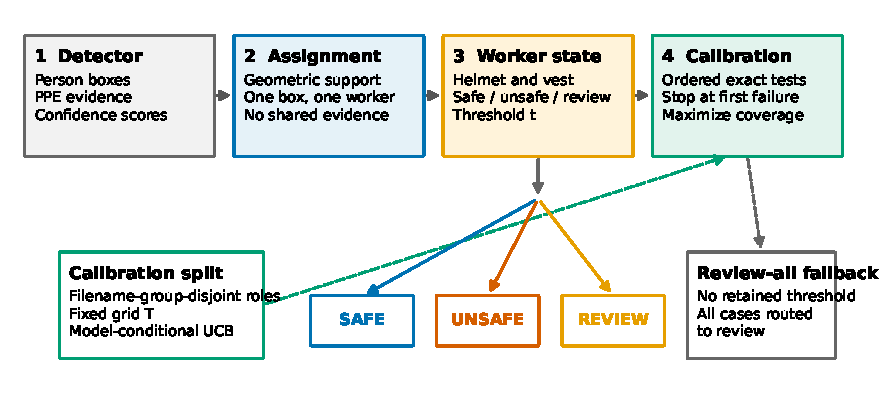
\includegraphics[width=\textwidth]{figures/v23/fig1_rc_wssi_pipeline.pdf}
\caption{RC-WSSI converts object detections into a geometry-defined single-owner representation. PPE evidence has one person owner, is mapped to safe/unsafe/review, and is evaluated under a declared filename-group-disjoint role split. The fixed high-to-low threshold diagnostic returns the most permissive retained threshold under its stated model; infeasible selection returns review-all. The full-corpus endpoint remains geometry-defined; a blinded, independently adjudicated human ownership audit is reported separately for the selected candidate-restricted multi-worker subset.}
\label{fig:pipeline}
\end{figure*}

\subsection{Worker-level task}

For image $X$, let $P=\{p_i\}_{i=1}^{m}$ be detected person boxes and let $E$ be helmet, vest, and violation detections. Each evaluable reference worker has state $Y_i\in\{\mathrm{safe},\mathrm{unsafe}\}$. Ambiguous or incomplete object annotations are retained as a descriptive review state but excluded from the binary risk denominator. The word ``reference'' is deliberate: the primary full-corpus worker-level state is generated by the predefined geometric association rule below. A separate blinded human audit evaluates PPE-to-worker ownership on a held-out multi-worker subset without replacing the full-corpus geometry-defined worker-state endpoint.

The detector used in our experiments follows the original annotation identifiers

\begin{equation}
\begin{aligned}
0&:\mathrm{helmet},\quad 1:\mathrm{no\ helmet},\quad 2:\mathrm{no\ vest},\\
3&:\mathrm{person},\quad 4:\mathrm{vest}.
\end{aligned}
\end{equation}

The final filename-grouped evaluator validates both checkpoint metadata and annotation geometry, then uses the original annotation map above. This audit is important because a display-name permutation can leave numeric training labels unchanged while corrupting downstream semantic interpretation.

\subsection{Assignment-conditioned PPE evidence}

For evidence box $e$ and person box $p_i$, we expand the person box by a factor of 1.15 and define

\begin{equation}
s(e,p_i)=\left(\frac{|e\cap \bar p_i|}{|e|},\;\operatorname{IoU}(e,\bar p_i),\;\mathbb{1}[c_e\in \bar p_i]\right),
\end{equation}

where $\bar p_i$ is the expanded box, $c_e$ is the arithmetic center of $e$, and IoU denotes intersection over union. Center support is binary and uses closed box boundaries: $\mathbb{1}[c_e\in\bar p_i]=1$ exactly when $\bar p_{i,x_1}\leq c_{e,x}\leq\bar p_{i,x_2}$ and $\bar p_{i,y_1}\leq c_{e,y}\leq\bar p_{i,y_2}$. An evidence box is eligible only when its first score component is positive or its center-support component is one; IoU alone cannot make it eligible. Among eligible persons, evidence is assigned to the lexicographically greatest support score. Exact score ties use the lowest current input person index. This is a single-owner, many-to-one allocation: each evidence box has at most one owner, while a person may receive multiple evidence boxes. Thus one detected helmet or vest is not copied to every person.

The evaluator applies the geometry to the detector-coordinate boxes as provided. A zero-area evidence box has no positive intersection and is therefore not eligible; the $10^{-9}$ area floor only prevents an arithmetic division by zero. Coordinates outside the image are not silently repaired by a separate clipping rule. Duplicate boxes that survive non-maximum suppression (NMS) remain separate evidence records and are assigned independently, with the stable person-index tie rule resolving exact geometric ties. If no person is eligible, the evidence has no owner and contributes no positive or negative confidence to any worker; the affected component consequently remains review. These edge cases are recorded by the evaluator rather than being converted into an artificial safe state.

Let $h_i^+$ and $h_i^-$ be the maximum assigned helmet and no-helmet confidences; $v_i^+$ and $v_i^-$ are defined analogously. For component confidence pair $(a^+,a^-)$ and threshold $t$, define

\begin{equation}
g_t(a^+,a^-)=
\begin{cases}
\mathrm{review}, & \max(a^+,a^-)<t,\\
\mathrm{unsafe}, & a^-\geq t\ \wedge\ a^-\geq a^+,\\
\mathrm{safe}, & a^+\geq t,\\
\mathrm{review}, & \text{otherwise}.
\end{cases}
\end{equation}

The worker state is unsafe if either component is unsafe, safe only if both components are safe, and review otherwise. Geometry-defined reference states use the same assignment geometry with binary label presence. Conflicting or incomplete component evidence is marked review rather than discarded from the released records. The primary binary summaries exclude these states, but we additionally report a conservative sensitivity that treats every reference-review worker as unsafe. Across the 30 repeated cells, the reference-review state occurs in 10,265 of 48,015 reference-person instances (21.4\%). Thus, the association rule is an explicit operational convention for constructing a worker-centric reference from object-level annotations; it is not presented as independently human-validated identity ground truth.

\subsection{Executable decision protocol}
The following compact pseudocode specifies the complete deterministic evaluator used for every cached prediction. It makes explicit the precedence of evidence states, the fallback policy, and the denominators used in the reported metrics.

\begin{quote}
\small
\textbf{Algorithm 1: Geometry-defined evidence allocation and risk reporting.}\\
\textbf{Input:} person boxes $P$, evidence boxes $E$, expansion $s=1.15$, threshold grid $\mathcal{T}_{\downarrow}$, target $(\alpha,\delta)$.\\
\textbf{Allocation:} for each $e\in E$, compute $q_i=(|e\cap\bar p_i|/|e|,\operatorname{IoU}(e,\bar p_i),\mathbf{1}[c_e\in\bar p_i])$. Discard $e$ when the first and third components are both zero. Assign every remaining $e$ to the lexicographically largest $q_i$; break an exact tie by the smallest person index.\\
\textbf{State rule:} for each person and component, let $(a^+,a^-)$ be the maximum assigned positive and negative confidences, with $0$ for an absent class. Return review if both are below $t$; otherwise return unsafe if $a^-\geq t$ and $a^-\geq a^+$; otherwise return safe if $a^+\geq t$; otherwise return review. At worker level, unsafe has precedence over safe, and safe requires both components safe; every other combination is review.\\
\textbf{Selection:} for $t$ in $\mathcal{T}_{\downarrow}$, count $n$ all-reference unsafe workers and $k_t$ automatic-safe errors, compute $U_t=\operatorname{Beta}^{-1}(1-\delta;k_t+1,n-k_t)$, and retain the prefix while $U_t\leq\alpha$. Select the most permissive retained threshold by the predeclared coverage tie-break; if none is retained, emit review-all.\\
\textbf{Reporting:} with $n_u$ all-reference unsafe workers, $e_a$ automatic-safe errors, and $e_m$ unmatched unsafe workers, report $R_{\mathrm{auto}}=e_a/n_u$, $R_{\mathrm{comp}}=(e_a+e_m)/n_u$, and $R_{\mathrm{match}}$ on matched unsafe workers only. Compute unsafe F1 from the explicitly defined TP/FP/FN counts; report coverage and prediction review using their separate denominators.\\
\end{quote}

\subsection{Selective objectives and reported scopes}

The implemented threshold-diagnostic event is automatic safe acceptance among all geometry-defined unsafe reference persons:

\begin{equation}
\begin{aligned}
R_{\mathrm{auto}}(t)
&=\Pr\{\pi_t(X,i)=\mathrm{safe}\\
&\qquad\mid Y_i=\mathrm{unsafe}\}.
\end{aligned}
\label{eq:risk}
\end{equation}

For an unmatched reference person, $\pi_t(X,i)$ is the detector-layer abstention symbol $\bot$, not a safe decision. Such persons remain in the denominator of $R_{\mathrm{auto}}$ but cannot contribute an automatic-safe error. We also report the matched-only diagnostic $R_{\mathrm{match}}(t)=\Pr\{\pi_t(X,i)=\mathrm{safe}\mid Y_i=\mathrm{unsafe},i\ \mathrm{matched}\}$ and the end-to-end quantity $R_{\mathrm{comp}}(t)=\Pr\{\pi_t(X,i)\in\{\bot,\mathrm{safe}\}\mid Y_i=\mathrm{unsafe}\}$, which counts both missed and automatically safe unsafe reference persons. For one common matched-worker population, automatic coverage and its complementary review probability are

\begin{equation}
\begin{aligned}
C_{\mathrm{m}}(t)&=\Pr\{\pi_t\in\{\mathrm{safe},\mathrm{unsafe}\}\mid \mathrm{matched}\},\\
Q_{\mathrm{m}}(t)&=1-C_{\mathrm{m}}(t).
\end{aligned}
\end{equation}

Given target $\alpha$, the procedure returns the most permissive threshold in the fixed sequence whose all-reference automatic-safe rate passes the model-conditional calculation. The matched and composite quantities are not used to select a threshold.

\subsection{Fixed-sequence model-conditional diagnostic}

Let the fixed grid be $t_1>\cdots>t_K$, explicitly ordered as $\mathcal{T}_{\downarrow}=(0.50,0.40,0.30,0.25,0.20,0.15,0.10,0.05)$. For $n$ unsafe calibration reference persons and $k_j$ automatic-safe errors at $t_j$, the one-sided exact upper confidence bound (UCB) is

\begin{equation}
U_j=\operatorname{Beta}^{-1}(1-\delta;k_j+1,n-k_j),
\label{eq:cp}
\end{equation}

with $U_j=1$ when $n=0$ or $k_j=n$. Starting at $t_1$, we retain $t_j$ when $U_j\leq\alpha$, continue only after retention, and stop at the first failure. Among retained thresholds, the implementation uses calibration coverage as the primary tie-break and the lower threshold as a stable secondary tie-break. If the first threshold fails, the policy routes every prediction to review. Since automatic-safe counts cannot decrease as the threshold is lowered and $n$ is fixed, $U_j$ cannot decrease either. Consequently, a full-grid ordinary CP scan with the same level retains this identical prefix; the ordered implementation is a transparent early-stop implementation rather than a distinct statistical selector.

\begin{proposition}[Nested safe sets]\label{prop:monotone}
Let $S(t)=\{(X,i):\pi_t(X,i)=\mathrm{safe}\}$. For any $t_{\mathrm{high}}\geq t_{\mathrm{low}}$, $S(t_{\mathrm{high}})\subseteq S(t_{\mathrm{low}})$. Equivalently, if $t_2\leq t_1$, then $S(t_1)\subseteq S(t_2)$. Therefore both $R_{\mathrm{auto}}(t)$ and $R_{\mathrm{match}}(t)$ are non-increasing as the threshold $t$ increases.
\end{proposition}

\begin{proof}
Consider a worker that is safe at $t_{\mathrm{high}}$. For each PPE component, its positive confidence is at least $t_{\mathrm{high}}$ and its negative confidence is strictly smaller than the positive confidence; otherwise the component would be unsafe at $t_{\mathrm{high}}$. Lowering the threshold can make a previously reviewed component automatic, but it cannot make this positive confidence lose to a negative confidence. Thus both components remain safe at $t_{\mathrm{low}}$, which proves the inclusion.
\end{proof}

\begin{proposition}[Model-conditional fixed-sequence calculation]\label{prop:ordered}
Assume the grid and order are fixed before calibration, unsafe calibration reference persons are exchangeable with deployment unsafe reference persons, and the automatic-safe indicators are independent Bernoulli trials with the binomial sampling law at each fixed threshold. Then the probability that the procedure returns any threshold with $R_{\mathrm{auto}}(t)>\alpha$ is at most $\delta$. This is explicitly a model-conditional statement: the four-way filename-group split removes declared cross-role overlap but does not prove independence among persons or frames within a filename group.
\end{proposition}

\begin{proof}
By Proposition~\ref{prop:monotone}, bad hypotheses $H_j:R_{\mathrm{auto}}(t_j)>\alpha$ form a suffix of the high-to-low sequence. A false retention requires rejection of the first true $H_j$. Its exact one-sided test has probability at most $\delta$ of rejection, and no later hypothesis is tested after a failure. Thus the stated model-conditional false-retention probability is at most $\delta$ without Bonferroni division.
\end{proof}

\subsection{Assignment contamination model}

Let $r_0$ be local unsafe-to-safe risk without foreign PPE evidence. Suppose foreign safe evidence triggers acceptance with probability $\rho$ conditional on no local error. If assignment fails with probability at most $\epsilon$ and the failure and contamination events are conditionally independent, then

\begin{equation}
\begin{aligned}
R_{\mathrm{global}}&=r_0+(1-r_0)\rho,\\
R_{\mathrm{assign}}&\leq r_0+(1-r_0)\epsilon\rho.
\end{aligned}
\label{eq:contamination}
\end{equation}

The model isolates cross-worker contamination. It does not cover missed person boxes or end-to-end detector failures. Semantic agreement between the allocation rules and human PPE ownership judgments is evaluated separately on the independently adjudicated audit subset described in Section~\ref{sec:humanprotocol}.

\section{Experimental protocol}\label{sec:experiments}

\subsection{Data and label budgets}

We use a five-class low-light tunnel PPE corpus containing 9,455 images and the classes helmet, no helmet, no reflective vest, person, and reflective vest. The same image source has been used in prior low-light tunnel PPE work \cite{wang2023lowlight}; our task, decision labels, filename grouping, and risk metrics are different. For each of five sampling seeds and three folds, the final protocol creates four filename-group-disjoint roles: detector training, detector validation, risk calibration, and final test. The 5\% and 10\% budgets refer to the fraction of each filename-group-restricted training pool used for detector training, not to 5\% or 10\% of the complete 9,455-image corpus. They are separately sampled experimental conditions rather than nested points on a learning curve. Across cells, training contains 100--122 images at 5\% and 200--244 images at 10\%; detector validation contains 289--410 images, calibration 290--430 images, and final test 1,392--1,631 images.

Filename groups are inferred by removing only the parenthesized frame index; for example, \texttt{8\_tunnel (102).jpg} and \texttt{8\_tunnel (103).jpg} map to \texttt{8\_tunnel}. Whole filename groups are assigned to exactly one of the four roles. The independent protocol audit found zero path overlap, zero filename-group overlap, and zero image-hash overlap for every pair of roles in all 30 cells. Per cell, the roles contain 3--4 training groups, 2 detector-validation groups, 2 calibration groups, and 3--4 final-test groups; across the three folds, the final-test role contains 11 unique filename groups. These identifiers are filename-derived proxies rather than verified video, camera, date, or worker-track identities, so we make only a filename-group-disjoint claim. Across the five seeds, each group assignment for a fold is deliberately reused; each final-test filename group appears in five cells at a given label budget. The 15 cell summaries are consequently repeated-training descriptions, not 15 independent deployment samples.

The calibration sample structure is reported separately from the image count because it determines how the exact calculation should be interpreted. Every calibration cell contains two filename groups, 290--430 calibration images, and 84--269 geometry-defined unsafe reference workers (median 228 across cells). These workers are not asserted to be independent trials: workers from the same group, and especially adjacent frames, may be correlated. Consequently, the split establishes role separation but not a group-level finite-sample guarantee. Proposition~\ref{prop:ordered} is therefore used only as a model-conditional worker-level diagnostic; a cluster-valid analysis would require verified video/track identifiers or a larger independent-group calibration design.

\subsection{Detector and implementation}

The primary detector is YOLOv8s implemented with Ultralytics 8.3.239 \cite{ultralytics2025}. To test detector dependence, we repeat the complete protocol with a second detector, YOLO11s, initialized from its corresponding pretrained weights. Both variants are fine-tuned for at most 100 epochs at $640\times640$ resolution with SGD ($lr_0=0.01$, $lrf=0.01$), patience 20, deterministic per-cell seeds, automatic mixed precision, and the fixed Ultralytics augmentations mosaic $=1.0$, scale $=0.5$, and horizontal flip $=0.5$; the primary run uses batch size 8 and the YOLO11s robustness run uses batch size 6 because it was executed as two coordinated GPU shards. For each seed--fold cell, \texttt{best.pt} is selected exclusively by mAP@0.50:0.95 on the detector-validation role. The calibration and final-test images are not loaded by the training process and cannot affect checkpoint selection. The selected validation row and checkpoint-stored metrics agree in all 30 cells for each detector.

\begin{table*}[t]
\caption{Detector-validation metrics at the saved best checkpoint. Values are means over 15 seed--fold cells with descriptive seed-resampling intervals in brackets; all three folds remain together. YOLOv8s is the primary detector and YOLO11s is the second-detector robustness run. These intervals quantify training-repeat variability, not population generalization. The object-level metrics characterize the detector input to RC-WSSI and are not covered by its conditional worker-state audit.}
\label{tab:detector}
\centering
\scriptsize
\setlength{\tabcolsep}{5pt}
\begin{tabular}{@{}c l c c c c@{}}
\toprule
Labels & Detector & Precision & Recall & mAP@0.50 & mAP@0.50:0.95 \\
\midrule
5\%  & YOLOv8s & 0.761 [0.743, 0.776] & 0.654 [0.641, 0.668] & 0.716 [0.709, 0.724] & 0.343 [0.336, 0.350] \\
5\%  & YOLO11s & 0.782 [0.766, 0.802] & 0.655 [0.643, 0.669] & 0.726 [0.716, 0.733] & 0.357 [0.350, 0.363] \\
10\% & YOLOv8s & 0.794 [0.789, 0.799] & 0.688 [0.678, 0.698] & 0.754 [0.748, 0.764] & 0.387 [0.381, 0.392] \\
10\% & YOLO11s & 0.797 [0.792, 0.802] & 0.676 [0.668, 0.686] & 0.754 [0.751, 0.759] & 0.391 [0.389, 0.394] \\
\bottomrule
\end{tabular}
\end{table*}

The YOLOv8s best validation epoch averages 78.3 (range 28--99) at 5\% labels and 73.4 (34--91) at 10\%; the YOLO11s averages 84.7 (72--98) and 72.8 (41--97), respectively. Inference uses a detection confidence floor of 0.05 and non-maximum suppression (NMS) IoU of 0.70. RC-WSSI then uses person matching IoU of 0.5, person expansion 1.15, and threshold grid

\begin{equation}
\mathcal{T}=\{0.05,0.10,0.15,0.20,0.25,0.30,0.40,0.50\}.
\end{equation}

This is an unordered set; the implementation scans it only in the descending order $\mathcal{T}_{\downarrow}$ stated in Section~3.3. The expansion factor $1.15$, person-match IoU $0.5$, prediction score floor $0.05$, and this threshold grid were fixed evaluator settings before final-test scoring. They were not optimized on final-test images; in this study they are engineering conventions rather than claims of independently optimized hyperparameters. The frozen-cache perturbation analysis below therefore tests operational sensitivity, not parameter optimality. Table~\ref{tab:detector} reports detector-validation metrics because this is the role used for checkpoint selection. Final-test detector outputs are held out and consumed only by the predeclared worker-state evaluator; the manuscript makes no standalone final-test object-detection generalization claim.

We set $\alpha=0.30$ and $\delta=0.10$ before evaluation. The relatively permissive target reflects a feasibility study under small calibration samples; it is not a recommended universal deployment value or a statement of end-to-end system safety.

\subsection{Comparisons and metrics}

We compare the proposed lexicographic allocation with center-inside, maximum-IoU, Hungarian-IoU, and global-pooling alternatives. The first three are local allocation rules; global pooling supplies every PPE box to every detected person. The analysis varies $\alpha\in\{0.05,0.10,0.20,0.30\}$, $\delta\in\{0.05,0.10\}$, and the reporting scope. The formal selection quantity is all-reference automatic-safe rate; matched-worker unsafe-to-safe and the composite event ``unsafe worker missed or accepted as safe'' are complementary diagnostics.

Predicted and reference persons are greedily matched at IoU 0.5 in descending prediction confidence. This pre-specified evaluator is supplemented by a frozen-cache Hungarian-IoU matching sensitivity analysis. Unmatched unsafe reference persons are detector-layer abstentions: they remain in the formal all-reference automatic-safe denominator, count as unsafe misses in the composite diagnostic, and are outside the matched-only diagnostic denominator. We report unsafe F1, all-reference automatic-safe rate, matched unsafe-to-safe rate, composite miss-or-safe rate, automatic coverage among matched persons, prediction review rate, unsafe miss rate, and the full safe/unsafe/review count vectors in the released per-cell CSVs. Coverage and prediction review rate are not complementary: coverage uses matched reference persons, whereas review rate uses all predicted persons.

For unsafe F1, a matched unsafe reference worker predicted unsafe is a true positive; a matched unsafe worker predicted safe or review, and an unmatched unsafe reference worker, are false negatives. A safe reference worker predicted unsafe and an unmatched or extra predicted unsafe worker are false positives. Review is not itself a false positive, but it reduces the number of unsafe workers counted as detected unsafe and therefore affects F1 through the preceding definition. The composite miss-or-safe risk counts both unmatched unsafe reference workers and automatically safe matched unsafe workers in its numerator.

Means are taken over 15 seed--fold cells for each label budget. Descriptive seed-resampling intervals use 5,000 percentile draws with the five sampling seeds as resampling units while retaining their three folds together. They summarize repeated-training variation, not a confidence interval for a target deployment population, because seeds and filename groups are reused. We therefore also release per-cell denominators/errors and report source-fold descriptive distributions after averaging the five seed repetitions. The final evaluator was rerun over all 30 rate--seed--fold cells after a class-metadata audit; it produced calibration and test prediction caches, filename-group membership records, selected-threshold records, fallback outcomes, and per-image records with no failed cells. All checkpoint decisions use detector validation, all threshold decisions use calibration, and final-test labels are used only once for held-out evaluation. The person expansion, matching IoU, detection floor, and threshold grid are fixed development settings across all cells; no independent hyperparameter-optimization claim is made for them, and their frozen-cache perturbation sensitivity is reported below.

\subsection{Blinded, independently adjudicated human association audit}\label{sec:humanprotocol}

We construct a source-balanced audit from the outer final-test role of the 10\% protocol before inspecting human labels or method accuracy. This is a selected candidate-restricted subset designed to stress ownership decisions in difficult multi-worker scenes; its results do not estimate full-corpus ownership prevalence. The audit contains 60 multi-worker images, 317 annotated person boxes, and 597 annotated PPE evidence boxes from all 11 filename groups. Selection uses only source balance, person count, person overlap, median person size, and the number of evidence boxes supported by more than one person; it does not use detector predictions, threshold outcomes, or human assignments. The audit therefore evaluates evidence ownership independently of detector recall and confidence. Because this set is deliberately difficult and candidate-restricted, it complements but does not estimate the ownership error rate of the full corpus.

Each image displays every person as \texttt{P1}, \texttt{P2}, and so forth and each PPE evidence box as \texttt{E1}, \texttt{E2}, and so forth. Candidate owner IDs include persons with positive expanded-box intersection or center support. Each expert chooses one candidate, \texttt{NONE}, or \texttt{AMBIGUOUS}; \texttt{NONE} permits rejection when no listed person owns the evidence. This candidate restriction makes the audit an ownership decision among geometrically plausible persons rather than unconstrained scene annotation and is retained as a limitation.

Two blinded annotators complete separate local annotation passes. The server exposes only the assigned expert's response file and rendered images; it does not expose the sealed proposed allocation or the other expert's responses. Each pass contains all 597 rows and is frozen with a SHA-256 digest before comparison. The primary inter-annotator result is row-wise exact agreement: 587/597 (98.32\%). Cohen's $\kappa=0.980$ is reported only as an auxiliary descriptor because candidate person IDs and their marginal distributions vary across audit rows; it is not treated as the primary reliability estimate. A third expert then sees only the 10 disagreements and the two initial choices, inspects the same image, and records the final owner. Adjudication confidence metadata are not used because they were optional and incomplete; only the frozen final owner label enters evaluation.

The four local rules and global pooling are replayed on the same annotated person and PPE boxes. Exact owner-set accuracy requires the predicted owner set to equal the adjudicated human set; an unowned human label is the empty set. For global pooling the predicted set contains every person in the image, so merely containing the true owner is not counted as correct. We additionally report owner-link precision, recall, and F1, image-macro and filename-group-macro accuracy, and descriptive paired filename-group resampling intervals from 20,000 draws. Filename groups are not verified independent videos, so these intervals describe stability to resampling the declared groups and are not cluster-valid population confidence intervals. The human labels are used only for this final audit and never for detector, parameter, or threshold selection.

\subsection{Complementary source-stratified random audit protocol}
To complement the deliberately difficult audit, we froze a second audit sample before inspecting detector predictions or method outcomes. The sample contains 66 outer-test images, exactly six from each of the 11 declared filename groups, and excludes all 60 images in the difficult audit. Within each group, images were sampled with fixed seed 20260812 after stratifying by annotated person count (single, 2--3, or 4+) and PPE-box count (1--4, 5--9, or 10+); the sampling code reads only the source-disjoint test manifest and human object boxes. The frozen package contains 334 PPE boxes and 217 person boxes. Before any human random-audit labels were inspected, we upgraded its protocol to three separate blind passes. For every PPE box, each expert could select any visible person ID displayed in that image, \texttt{NONE}, or \texttt{AMBIGUOUS}; the original geometric candidate list was retained only to report post hoc candidate-set recall, not to constrain the answer. Experts A, B, and C did not see detector predictions, thresholds, rule outputs, or each other's responses. All three passes were frozen before comparison. They produced 299/334 three-way exact agreements (89.52\%), pairwise exact agreement of 92.81\% (A--B), 91.92\% (A--C), and 94.01\% (B--C), and one three-way split retained as \texttt{AMBIGUOUS} by the predeclared rule. The resulting reference contains 321 determinate rows and 13 ambiguous rows. The original geometric candidate set contains the human owner in 320/321 determinate rows (99.69\% candidate-set recall), with one determinate human owner outside that set. This protocol provides complementary sampled ownership evidence; it cannot retroactively turn the geometry-defined full-corpus reference into a full semantic ground truth.


For qualitative analysis, we define four archetypes before rendering: a clean correct single-worker decision, a clean mixed-state multi-worker decision, a case where global pooling adds unsafe-to-safe errors, and a matched worker sent to review. Deterministic rankings use person area or case severity followed by fixed metadata tie-breaks. The displayed examples are an illustrative filename-group-disjoint evaluation-side visual audit, not a full-corpus semantic annotation study. Their candidate counts, paths, thresholds, and outcomes are archived separately, and they are not used to tune the detector or threshold.

\section{Results}\label{sec:results}

\subsection{Main and conservative filename-grouped results}

\begin{table*}[t]
\caption{Worker-state \emph{cell-mean} results under the declared four-role filename-group-disjoint protocol. Every rate is the unweighted mean over 15 repeated seed--fold cells, not a pooled-person rate or an independent deployment estimate. Auto-safe is the formal selection scope: automatic-safe errors divided by all unsafe reference persons. Composite is miss-or-safe over the same denominator; Missed is the unmatched unsafe-reference rate. Coverage is matched-person coverage, whereas Review is the prediction-level review rate. Fallbacks are review-all outcomes. Person-weighted pooled rates and their counts are reported separately in Table~\ref{tab:estimands}; no entry is a cluster-valid confidence bound.}
\label{tab:main}
\centering
\scriptsize
\setlength{\tabcolsep}{2.5pt}
\begin{tabular}{@{}c l c c c c c c c@{}}
\toprule
Labels & Method & Unsafe F1 & Auto-safe & Composite & Missed & Coverage & Review & Fallbacks \\
\midrule
5\% & Center-inside & 0.683 & 0.137 & 0.206 & 0.069 & 0.795 & 0.379 & 0/15 \\
5\% & Max-IoU & 0.673 & 0.134 & 0.202 & 0.069 & 0.779 & 0.375 & 0/15 \\
5\% & Hungarian-IoU & 0.671 & 0.132 & 0.201 & 0.069 & 0.786 & 0.364 & 0/15 \\
5\% & Global pooling & 0.215 & 0.111 & 0.180 & 0.069 & 0.385 & 0.618 & 9/15 \\
5\% & RC-WSSI & 0.677 & 0.136 & 0.205 & 0.069 & 0.791 & 0.375 & 0/15 \\
\midrule
10\% & Center-inside & 0.731 & 0.113 & 0.173 & 0.060 & 0.827 & 0.324 & 0/15 \\
10\% & Max-IoU & 0.722 & 0.111 & 0.171 & 0.060 & 0.817 & 0.321 & 0/15 \\
10\% & Hungarian-IoU & 0.723 & 0.112 & 0.172 & 0.060 & 0.828 & 0.308 & 0/15 \\
10\% & Global pooling & 0.280 & 0.114 & 0.174 & 0.060 & 0.450 & 0.552 & 8/15 \\
10\% & RC-WSSI & 0.727 & 0.112 & 0.172 & 0.060 & 0.825 & 0.320 & 0/15 \\
\botrule
\end{tabular}
\end{table*}

The cell-mean RC-WSSI values in Table~\ref{tab:main} must not be reconstructed by dividing counts pooled across the 15 repeated cells. The pooled denominators, automatic-safe errors, and unmatched-unsafe events are now reported explicitly in Table~\ref{tab:estimands}. These pooled records contain 17,945 unsafe reference-person instances at each label condition; at 5\% they contain 2,866 automatic-safe and 1,161 unmatched-unsafe events, and at 10\% they contain 2,321 and 984 events. They produce the \emph{person-weighted} rates $0.160/0.224$ and $0.129/0.184$ (auto-safe/composite), respectively, rather than the cell means in Table~\ref{tab:main}. The repeated counts reuse filename groups across seeds and are not independent worker samples.

\begin{table*}[t]
\caption{Conservative reference-definition sensitivity reported alongside the cell-mean primary results: reference-review workers are treated as unsafe during both calibration selection and held-out evaluation, including the review-all fallback decision. This revision-added analysis was not a pre-specified co-primary endpoint. Values are means over 15 repeated seed--fold cells at $(\alpha,\delta)=(0.30,0.10)$; they are not semantic-association validation or deployment confidence bounds.}
\label{tab:reviewunsafe}
\centering
\scriptsize
\setlength{\tabcolsep}{5pt}
\begin{tabular}{@{}c c c c c c c@{}}
\toprule
Labels & Auto-safe & Composite & Coverage & Review & Fallbacks & Cells \\
\midrule
5\%  & 0.165 & 0.331 & 0.794 & 0.372 & 0/15 & 15 \\
10\% & 0.151 & 0.305 & 0.825 & 0.320 & 0/15 & 15 \\
\bottomrule
\end{tabular}
\end{table*}

At 10\%, the proposed rule is close to the local geometric alternatives: center-inside reaches F1 $0.731$ and coverage $0.827$, while RC-WSSI reaches F1 $0.727$ and coverage $0.825$. This result does not support a claim of universal superiority for the lexicographic score. Its value is that it is deterministic, single-owner, and inspectable, while maintaining the same operating regime as the other local rules. Global pooling is qualitatively different: it reduces unsafe F1 to $0.280$, lowers coverage to $0.450$, and triggers review-all in 8/15 cells.

The separately sampled 5\% condition has the same pattern. The proposed rule reaches F1 $0.677$, all-reference automatic-safe rate $0.136$, composite rate $0.205$, and coverage $0.791$ with no fallbacks, whereas global pooling triggers 9/15 fallbacks and its unsafe F1 falls to $0.215$. Because the 5\% and 10\% training subsets are not nested, these are separate experimental conditions rather than a strict annotation learning curve.

\subsection{Second-detector robustness}

Table~\ref{tab:detector_robustness} reports the complete filename-group-disjoint YOLO11s rerun using the same 30 training, calibration, and final-test cells. At 10\% labels, YOLO11s produces worker-state F1 $0.719$, all-reference automatic-safe rate $0.104$, composite rate $0.169$, and coverage $0.803$, compared with $0.727/0.112/0.172/0.825$ for YOLOv8s. At 5\%, the corresponding YOLO11s values are $0.681/0.129/0.200/0.802$, compared with $0.677/0.136/0.205/0.791$. No YOLO11s cell returned review-all at the primary $(\alpha,\delta)=(0.30,0.10)$ setting. The small changes in F1, risk, and coverage show that the worker-conditioned operating pattern is not tied to a single YOLO implementation, while the differences also make clear that this is detector-variant robustness rather than external-dataset validation.

\begin{table*}[t]
\caption{Worker-state robustness to a second detector under the same filename-group-disjoint protocol. Values are means over 15 seed--fold cells at the primary $\alpha=0.30$, $\delta=0.10$ setting. Auto-safe is the all-reference automatic-safe rate used for calibration; composite includes unmatched unsafe reference persons.}
\label{tab:detector_robustness}
\centering
\scriptsize
\setlength{\tabcolsep}{5pt}
\begin{tabular}{@{}c l c c c c c@{}}
\toprule
Labels & Detector & Unsafe F1 & Auto-safe & Composite & Coverage & Fallbacks \\
\midrule
5\%  & YOLOv8s  & 0.677 & 0.136 & 0.205 & 0.791 & 0/15 \\
5\%  & YOLO11s  & 0.681 & 0.129 & 0.200 & 0.802 & 0/15 \\
10\% & YOLOv8s  & 0.727 & 0.112 & 0.172 & 0.825 & 0/15 \\
10\% & YOLO11s  & 0.719 & 0.104 & 0.169 & 0.803 & 0/15 \\
\bottomrule
\end{tabular}
\end{table*}


\subsection{Conditional threshold-diagnostic sensitivity}

The reference-review-as-unsafe analysis below is a post hoc sensitivity introduced during manuscript revision. It repeats threshold selection and held-out scoring under a conservative relabeling; it is not a confirmatory endpoint and was not used to define the original operating point.

\begin{table*}[t]
\caption{Strictness and review-workload sensitivity of the model-conditional selection calculation at $\delta=0.10$. Auto-safe is the all-reference automatic-safe rate used in calibration; Composite is miss-or-safe risk over all unsafe reference persons; Safe$\rightarrow$unsafe is the false-alarm burden among safe reference persons. Values are means over 15 repeated seed--fold cells, not deployment confidence intervals.}
\label{tab:sensitivity}
\centering
\scriptsize
\setlength{\tabcolsep}{3pt}
\begin{tabular}{@{}ccrrrrrrr@{}}
\toprule
Labels & $\alpha$ & Unsafe F1 & Auto-safe & Composite & Coverage & Review & Safe$\rightarrow$unsafe & Fallbacks \\
\midrule
5\% & 0.05 & 0.086 & 0.004 & 0.072 & 0.065 & 0.953 & 0.008 & 13/15 \\
5\% & 0.10 & 0.324 & 0.024 & 0.093 & 0.292 & 0.784 & 0.032 & 8/15 \\
5\% & 0.20 & 0.583 & 0.079 & 0.148 & 0.644 & 0.496 & 0.081 & 2/15 \\
5\% & 0.30 & 0.677 & 0.136 & 0.205 & 0.791 & 0.375 & 0.092 & 0/15 \\
\midrule
10\% & 0.05 & 0.227 & 0.013 & 0.073 & 0.222 & 0.827 & 0.044 & 10/15 \\
10\% & 0.10 & 0.528 & 0.050 & 0.110 & 0.530 & 0.570 & 0.067 & 4/15 \\
10\% & 0.20 & 0.724 & 0.097 & 0.157 & 0.789 & 0.356 & 0.093 & 0/15 \\
10\% & 0.30 & 0.727 & 0.112 & 0.172 & 0.825 & 0.320 & 0.096 & 0/15 \\
\bottomrule
\end{tabular}
\end{table*}

Table~\ref{tab:sensitivity} makes the safety--workload trade-off explicit. At the strict $\alpha=0.05$ target, review-all occurs in 13/15 cells at 5\% and 10/15 at 10\%, with prediction review rates of $0.953$ and $0.827$. At $\alpha=0.10$, the corresponding fallback counts are 8/15 and 4/15. At $\delta=0.05$, the strict $\alpha=0.05$ calculation returns review-all in 14/15 and 12/15 cells, respectively; the complete $\alpha$--$\delta$ grid is released. Thus $\alpha=0.30$ is a feasibility operating point, not a domain-justified safety target or deployment recommendation.

The strict-target result is operationally sparse: only 2/15 cells at 5\% and 5/15 at 10\% retain a threshold at $\alpha=0.05$, with the remaining cells returning review-all. This availability rate is part of the result, not an implementation detail.

\begin{table*}[t]
\caption{Strict $\alpha=0.05$, $\delta=0.10$ results restricted to cells that retained a threshold rather than returning review-all. This retained-policy view is reported separately because the low all-cell means in Table~\ref{tab:sensitivity} are largely produced by review-all outcomes. Values are descriptive means only.}
\label{tab:strictretained}
\centering
\scriptsize
\setlength{\tabcolsep}{5pt}
\begin{tabular}{@{}c c c c c c c@{}}
\toprule
Labels & Retained cells & Auto-safe & Composite & Coverage & Review & Unsafe F1 \\
\midrule
5\%  & 2/15 & 0.027 & 0.101 & 0.491 & 0.648 & 0.642 \\
10\% & 5/15 & 0.039 & 0.114 & 0.667 & 0.481 & 0.681 \\
\bottomrule
\end{tabular}
\end{table*}

The retained-policy view in Table~\ref{tab:strictretained} prevents interpreting review-all as an automatically usable low-risk policy. Only 2/15 cells at 5\% and 5/15 at 10\% retain a threshold at $\alpha=0.05$; even among those retained cells, composite risk remains $0.101$ and $0.114$ because detector-layer unsafe misses are outside the automatic-safe selection event.

For the primary 10\% setting, the selected-threshold record is compact enough to report in full. Table~\ref{tab:selectedthresholds} gives the calibration unsafe-worker count $n$, automatic-safe error count $k$, model-based one-sided upper bound $U$, selected threshold, and fallback state for every seed--fold cell. The repeated choice of $t=0.05$ is an observed operating-point result, not evidence that the grid parameter is universally optimal.

\begin{table*}[t]
\caption{Per-cell threshold-selection audit for the primary 10\% YOLOv8s condition at $(\alpha,\delta)=(0.30,0.10)$. $n$ and $k$ are calibration counts, $U$ is the model-conditional Clopper--Pearson upper bound, and fallback means that no threshold was retained. These 15 rows reuse filename groups across seeds and are not independent deployment samples.}
\label{tab:selectedthresholds}
\centering
\scriptsize
\setlength{\tabcolsep}{5pt}
\begin{tabular}{@{}c c r r c c c@{}}
\toprule
Seed & Fold & $n$ & $k$ & $U$ & Selected $t$ & Fallback \\
\midrule
0 & 0 & 84  & 8  & 0.1501 & 0.05 & No \\
0 & 1 & 269 & 61 & 0.2628 & 0.05 & No \\
0 & 2 & 228 & 13 & 0.0821 & 0.05 & No \\
1 & 0 & 84  & 4  & 0.0929 & 0.05 & No \\
1 & 1 & 269 & 49 & 0.2159 & 0.05 & No \\
1 & 2 & 228 & 9  & 0.0616 & 0.05 & No \\
2 & 0 & 84  & 8  & 0.1501 & 0.05 & No \\
2 & 1 & 269 & 57 & 0.2472 & 0.05 & No \\
2 & 2 & 228 & 13 & 0.0821 & 0.05 & No \\
3 & 0 & 84  & 15 & 0.2438 & 0.05 & No \\
3 & 1 & 269 & 38 & 0.1724 & 0.05 & No \\
3 & 2 & 228 & 26 & 0.1458 & 0.05 & No \\
4 & 0 & 84  & 3  & 0.0778 & 0.05 & No \\
4 & 1 & 269 & 53 & 0.2316 & 0.05 & No \\
4 & 2 & 228 & 17 & 0.1020 & 0.05 & No \\
\bottomrule
\end{tabular}
\end{table*}

The monotonicity above changes the interpretation of calibration comparisons. A full-grid ordinary CP scan and the fixed-sequence calculation retain the same threshold prefix here, rather than constituting competing methods. We therefore do not claim an empirical power gain for the ordered implementation. Bonferroni, fixed-threshold, and calibration-F1 diagnostics are retained in the reproducibility package as operating-point descriptions, but are not used as evidence of a finite-sample guarantee. For transparency, every cell's selected threshold, auto-safe error count, all-unsafe denominator, fallback status, and model-based UCB are released; neither a cell mean nor a mean UCB is interpreted as a population confidence bound. Because each calibration cell has only two filename groups, these calculations cannot empirically verify the worker-level binomial assumption.

The two assignment summaries answer different questions. Table~\ref{tab:main} reports each method at its own selected operating point, including the effect of calibration and review-all fallback. Table~\ref{tab:fixed_assignment} fixes $t=0.05$ for every method and therefore isolates the evidence-allocation mechanism before threshold-selection differences are introduced.

\begin{table*}[t]
\caption{Fixed-threshold assignment comparison at $t=0.05$ for the 10\% setting. All methods use the same cached predictions and threshold, so this analysis separates evidence allocation from calibration selection. ``All-ref safe rate'' divides unsafe-to-safe errors by all unsafe geometry-defined reference persons, the same scope used for the model-conditional selection calculation. Values are means over 15 repeated seed--fold cells.}
\label{tab:fixed_assignment}
\centering
\small
\begin{tabular}{@{}lccccc@{}}
\toprule
Method & Unsafe F1 & All-ref safe rate & Composite & Coverage & Review \\
\midrule
Center-inside & 0.731 & 0.113 & 0.173 & 0.827 & 0.324 \\
Max-IoU & 0.722 & 0.111 & 0.171 & 0.817 & 0.321 \\
Hungarian-IoU & 0.723 & 0.112 & 0.172 & 0.828 & 0.308 \\
Global pooling & 0.573 & 0.240 & 0.300 & 0.980 & 0.024 \\
RC-WSSI & 0.727 & 0.112 & 0.172 & 0.825 & 0.320 \\
\bottomrule
\end{tabular}
\end{table*}

Table~\ref{tab:fixed_assignment} removes the calibration-selection confound. With all methods evaluated at $t=0.05$, the local rules remain close, whereas global pooling raises the common-denominator automatic-safe diagnostic to $0.240$ and composite risk to $0.300$ despite near-complete automatic coverage. Thus the supported claim is not that the lexicographic score is the best local matcher; rather, assigning each PPE observation before forming a worker state prevents the all-to-all evidence-sharing mechanism of global pooling.

To make the selected-policy comparison auditable, Table~\ref{tab:pairedallocation} and Fig.~\ref{fig:pairedallocation} report the paired 10\% results for all 11 filename-group/fold units. Each unit averages five seed repetitions. Differences are RC-WSSI minus global pooling; negative values favor RC-WSSI for that diagnostic. The table reports the unsafe-reference denominator per seed and each method's retained-threshold set together with the number of non-fallback seeds. A review-all seed has no selected threshold: its internal evaluator placeholder is never reported as a retained value. RC-WSSI has a lower composite rate in 5/11 units, while global pooling has at least one review-all seed in 7/11 units; this mixed pattern is why the paired analysis is descriptive evidence about ownership and feasibility, not a claim that RC-WSSI is uniformly superior at the selected operating point.

\begin{table*}[t]
\caption{Paired selected-policy comparison for the 10\% condition over all 11 filename-group/fold units. Each unit averages five seed repetitions. $\Delta$ is RC-WSSI minus global pooling; negative values favor RC-WSSI. Unsafe $n$ is the number of geometry-defined unsafe reference persons per seed. ``Retained $t$ [seeds]'' gives the set of distinct retained thresholds among the indicated non-fallback seeds; a review-all seed has no selected threshold, and ``-- [0/5]'' means every seed fell back. These are descriptive repeated-training summaries, not independent group-level inference.}
\label{tab:pairedallocation}
\centering
\scriptsize
\setlength{\tabcolsep}{3pt}
\resizebox{\textwidth}{!}{%
\begin{tabular}{@{}c l r c c r r@{}}
\toprule
Fold & Filename group & Unsafe $n$ & RC retained $t$ [seeds] & Pool retained $t$ [seeds] & $\Delta$ auto-safe & $\Delta$ composite \\
\midrule
0 & \texttt{11\_tunnel} & 421 & 0.05 [5/5] & -- [0/5] & 0.086 & 0.086 \\
0 & \texttt{5\_tunnel}  & 43  & 0.05 [5/5] & -- [0/5] & 0.042 & 0.042 \\
0 & \texttt{6\_tunnel}  & 152 & 0.05 [5/5] & -- [0/5] & 0.029 & 0.029 \\
0 & \texttt{8\_tunnel}  & 194 & 0.05 [5/5] & -- [0/5] & 0.020 & 0.020 \\
1 & \texttt{1\_tunnel}  & 7   & 0.05 [5/5] & \{0.05,0.40\} [2/5] & 0.057 & 0.057 \\
1 & \texttt{2\_tunnel}  & 34  & 0.05 [5/5] & \{0.05,0.40\} [2/5] & -0.029 & -0.029 \\
1 & \texttt{9\_tunnel}  & 1636& 0.05 [5/5] & \{0.05,0.40\} [2/5] & 0.079 & 0.079 \\
2 & \texttt{10\_tunnel} & 34  & 0.05 [5/5] & 0.05 [5/5] & -0.376 & -0.376 \\
2 & \texttt{3\_tunnel}  & 117 & 0.05 [5/5] & 0.05 [5/5] & -0.142 & -0.142 \\
2 & \texttt{4\_tunnel}  & 50  & 0.05 [5/5] & 0.05 [5/5] & -0.260 & -0.260 \\
2 & \texttt{7\_tunnel}  & 901 & 0.05 [5/5] & 0.05 [5/5] & -0.124 & -0.124 \\
\bottomrule
\end{tabular}}
\end{table*}

\begin{figure*}[t]
\centering
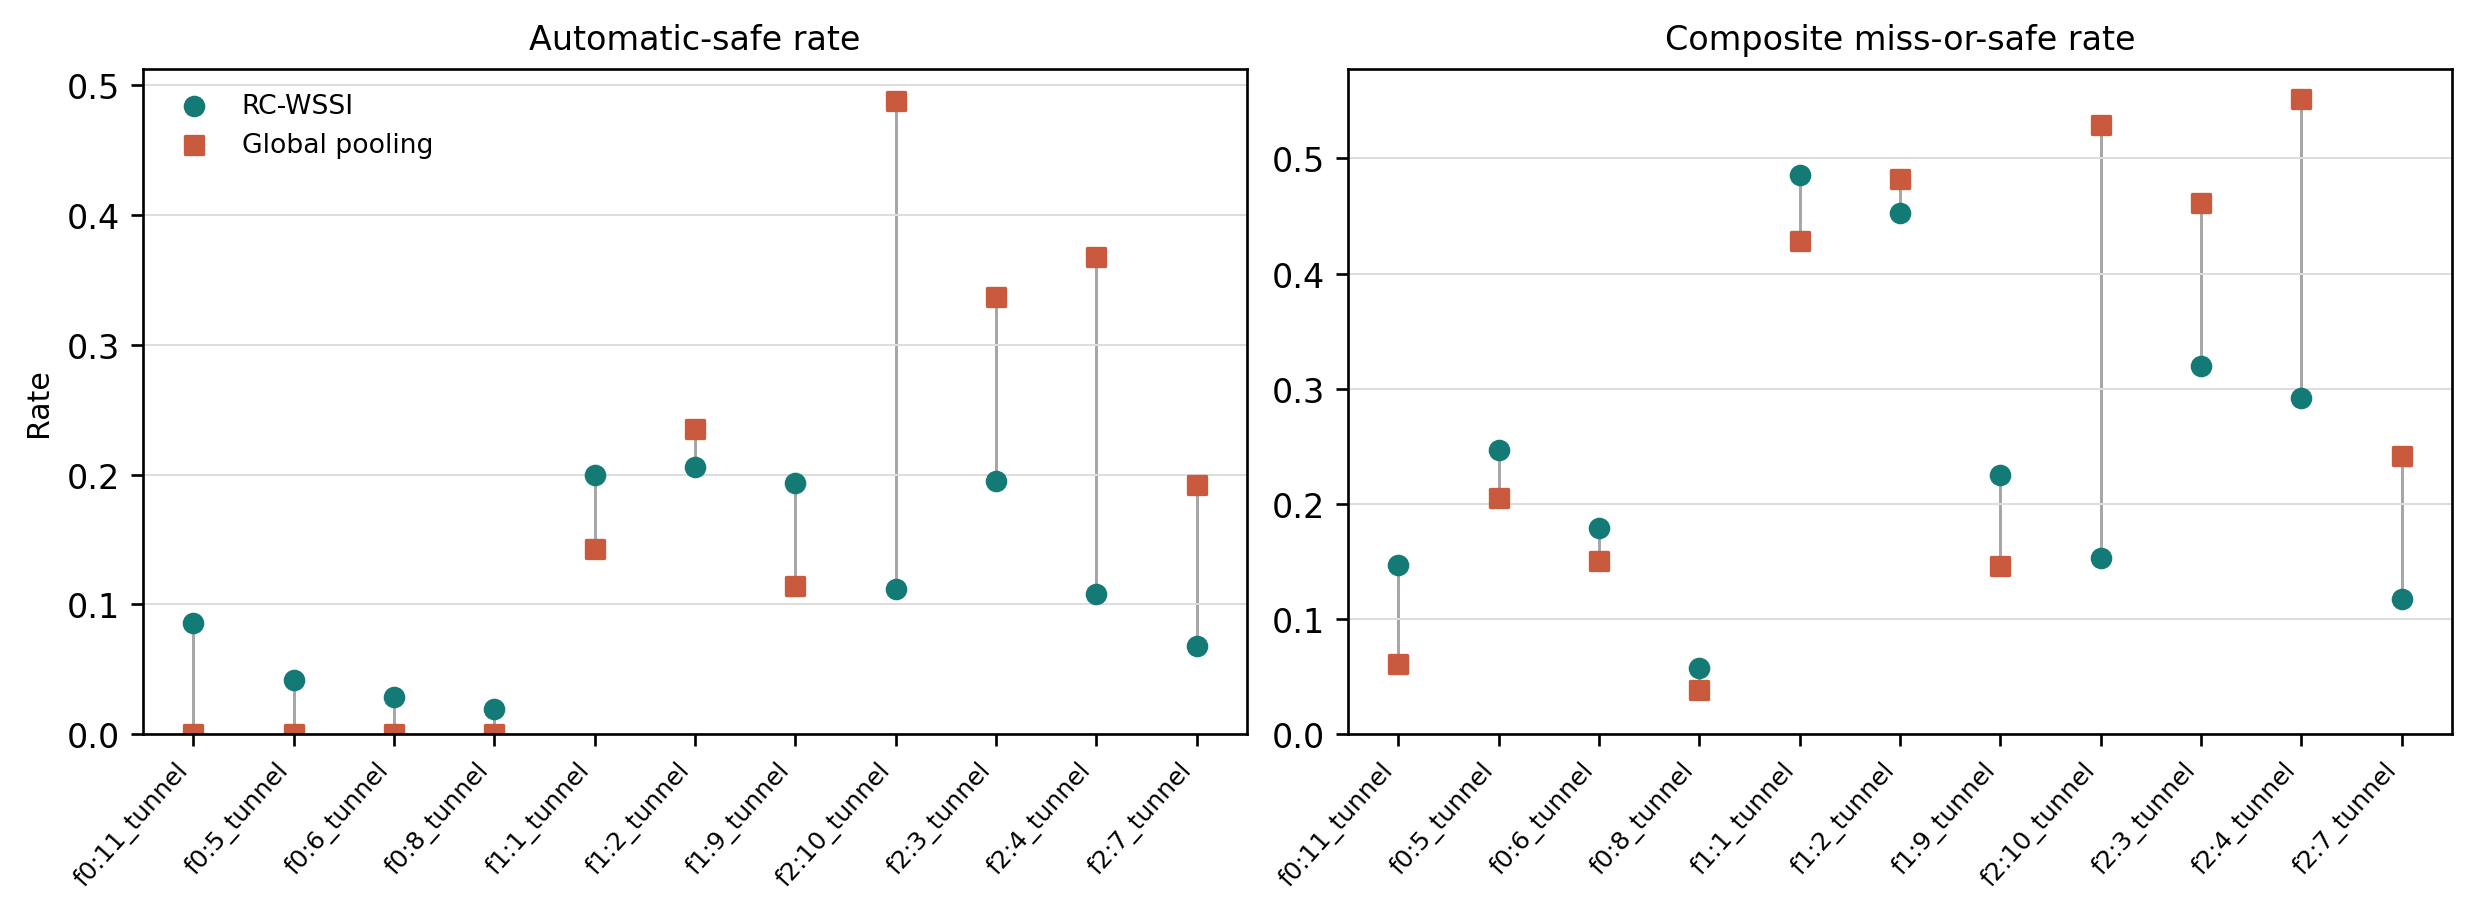
\includegraphics[width=0.96\textwidth]{figures/v23/fig6_selected_allocation_pairs.png}
\caption{Paired selected-policy rates for the 11 filename-group/fold units at 10\%, after averaging five seed repetitions. Gray segments connect RC-WSSI and global pooling within a unit. The plot is descriptive and includes the effect of method-specific threshold selection and review-all fallback; it is not a cluster-valid uncertainty display.}
\label{fig:pairedallocation}
\end{figure*}

\subsection{Reference-review and filename-group variability}

The 21.4\% reference-review share is treated as a main interpretive result alongside the default binary-reference summary: at 10\%, the default cell-mean composite is $0.172$, whereas the revision-added conservative review-as-unsafe recalculation is $0.305$. It treats every reference-review worker as unsafe during \emph{both} calibration selection and held-out evaluation, including the review-all fallback decision. This revision-added analysis was not declared as a co-primary endpoint before the original analysis. The primary 10\% condition then has automatic-safe rate $0.151$ and composite miss-or-safe rate $0.305$; the corresponding 5\% values are $0.165$ and $0.331$. These are deliberately harsher than the binary-reference values in Table~\ref{tab:main}, because ambiguous or incomplete reference relations are counted as safety-critical. They demonstrate that the numerical conclusion is sensitive to the geometry-defined reference convention and do not validate PPE-to-worker semantic identity. They are reported as a post hoc conservative sensitivity rather than silently promoted to a pre-specified primary endpoint.

Table~\ref{tab:sourcefold} exposes heterogeneity hidden by the 15 repeated seed--fold means. We first average each filename-group/fold result across its five seed repetitions, then summarize the 11 resulting filename-group/fold units. There are 11 rather than 15 because the final-test role contains 11 unique filename groups across the three folds; each unit is averaged over the five training seeds. These are descriptive distributions, not source-level confidence intervals: filename groups are proxies rather than verified independent videos, and the same corpus is reused across conditions. The observed 10\% composite minimum--maximum range is $0.058$--$0.486$ across the 11 units, so the mean $0.172$ does not describe the worst observed filename-group/fold unit. The worst 10\% unit is fold 1, \texttt{1\_tunnel}: 115 test images and 7 unsafe reference persons per seed (35 across five seeds), with 7 auto-safe errors and 10 unmatched-unsafe errors in aggregate, i.e. $17/35=0.486$. This is an aggregate across five repeated training runs, not 35 independent worker samples.

\begin{table*}[t]
\caption{Descriptive filename-group/fold distribution at the primary operating point after averaging the five seed repetitions within each unit. Entries are median [minimum, maximum] across 11 filename-group/fold units, not confidence intervals. The unit-size columns give median [minimum, maximum] images and unsafe-reference persons. Auto-safe and Composite use all unsafe reference persons as denominator. Complete worst-first unit rows, group names, denominators, unsafe-to-safe errors, and unmatched-unsafe counts are released with the audit artifact.}
\label{tab:sourcefold}
\centering
\scriptsize
\setlength{\tabcolsep}{4pt}
\resizebox{\textwidth}{!}{%
\begin{tabular}{@{}c c c c c c c c c@{}}
\toprule
Labels & Units & Images/unit & Unsafe/unit & Unsafe F1 & Auto-safe & Composite & Coverage & Review \\
\midrule
5\% & 11 & 155 [104, 1207] & 34 [7, 1636] & 0.545 [0.000, 0.905] & 0.079 [0.020, 0.251] & 0.205 [0.057, 0.457] & 0.786 [0.621, 0.919] & 0.404 [0.254, 0.491] \\
10\% & 11 & 155 [104, 1207] & 34 [7, 1636] & 0.577 [0.110, 0.923] & 0.108 [0.020, 0.206] & 0.225 [0.058, 0.486] & 0.772 [0.675, 0.928] & 0.352 [0.263, 0.436] \\
\bottomrule
\end{tabular}
}
\end{table*}

\begin{table*}[t]
\caption{Descriptive estimand sensitivity over the 11 unique filename-group/fold final-test units, after averaging the five seed repetitions within each unit. Each rate pair is auto-safe/composite. The cell mean is the repeated seed--fold estimand used in Table~\ref{tab:main}; person-weighted values pool unsafe reference-person counts across the 11 units; group-macro values give every filename-group/fold unit equal weight. Pooled $n_u$, $e_a$, and $e_m$ are the repeated-record unsafe denominator, automatic-safe errors, and unmatched-unsafe errors used for person-weighted rates. None is a cluster-valid deployment estimate. Reviews/image is reported in the text.}
\label{tab:estimands}
\centering
\small
\setlength{\tabcolsep}{3pt}
\begin{tabular}{@{}c c c c r r r@{}}
\toprule
Labels & Cell mean & Person weighted & Group macro & Pooled $n_u$ & Auto $e_a$ & Unmatched $e_m$ \\
\midrule
5\%  & 0.136 / 0.205 & 0.160 / 0.224 & 0.107 / 0.256 & 17,945 & 2,866 & 1,161 \\
10\% & 0.112 / 0.172 & 0.129 / 0.184 & 0.114 / 0.243 & 17,945 & 2,321 & 984 \\
\bottomrule
\end{tabular}
\end{table*}

The primary estimand is the mean over 15 repeated seed--fold cells, which describes training-repeat behavior under the fixed protocol. The additional person-weighted and group-macro summaries show that the headline cell mean is not a unique deployment estimand: at 10\%, the group-macro composite is $0.243$ and the worst filename-group/fold composite is $0.486$. The source-fold table and released raw rows give each unit's image count, unsafe-reference denominator, automatic-safe errors, and unmatched-unsafe errors. Reviews/image is $1.013$ at 5\% and $0.809$ at 10\%; the available metadata contain no frame rate or exposure duration, so a review-per-hour workload cannot be inferred.

The three folds contain the following filename groups in the final-test role: fold 0 has \texttt{5\_tunnel}, \texttt{6\_tunnel}, \texttt{8\_tunnel}, and \texttt{11\_tunnel}; fold 1 has \texttt{1\_tunnel}, \texttt{2\_tunnel}, and \texttt{9\_tunnel}; fold 2 has \texttt{3\_tunnel}, \texttt{4\_tunnel}, \texttt{7\_tunnel}, and \texttt{10\_tunnel}. These are filename groups, not verified video or worker identities.

\subsection{Blinded, independently adjudicated human-reference association results}\label{sec:humanresults}

The primary inter-annotator result is row-wise exact agreement: 587 of 597 PPE assignments (98.32\%). Cohen's $\kappa=0.980$ is an auxiliary descriptor only because candidate person IDs and their marginal distributions vary across audit rows. A third expert resolves all 10 disagreements, yielding a complete final reference with 589 person-owner labels and eight \texttt{NONE} labels; no final row remains \texttt{AMBIGUOUS}. The initial agreement is reported before adjudication and is not recomputed from the consensus labels.

\begin{table*}[t]
\caption{Assignment accuracy against the final human reference produced by separate blinded annotation passes and third-expert adjudication on the selected candidate-restricted subset of 60 multi-worker images and 597 PPE evidence boxes. Exact requires equality of the complete owner set. Intervals in brackets are descriptive filename-group resampling intervals from 20,000 draws, not cluster-valid confidence intervals. Image and Group are macro accuracies; Link P/R/F1 scores individual predicted owner links. Global pooling predicts every person as an owner and is included only to isolate all-to-all evidence sharing.}
\label{tab:humanaudit}
\centering
\scriptsize
\setlength{\tabcolsep}{3.5pt}
\resizebox{\textwidth}{!}{%
\begin{tabular}{@{}l r c c c c c r@{}}
\toprule
Method & Exact & Box accuracy [group resampling] & Image macro & Group macro & Link P/R/F1 & Extra links & Missed links \\
\midrule
RC-WSSI lexicographic & 582/597 & 0.975 [0.963, 0.984] & 0.977 & 0.977 & 0.975/0.985/0.980 & 15 & 9 \\
Center-inside & 580/597 & 0.972 [0.949, 0.983] & 0.970 & 0.965 & 0.971/0.978/0.975 & 17 & 13 \\
Hungarian-IoU & 575/597 & 0.963 [0.944, 0.995] & 0.967 & 0.976 & 0.968/0.969/0.969 & 19 & 18 \\
Max-IoU & 556/597 & 0.931 [0.913, 0.958] & 0.929 & 0.938 & 0.931/0.941/0.936 & 41 & 35 \\
Global pooling & 0/597 & 0.000 [0.000, 0.000] & 0.000 & 0.000 & 0.171/1.000/0.291 & 2,864 & 0 \\
\bottomrule
\end{tabular}}
\end{table*}

\begin{figure*}[t]
\centering
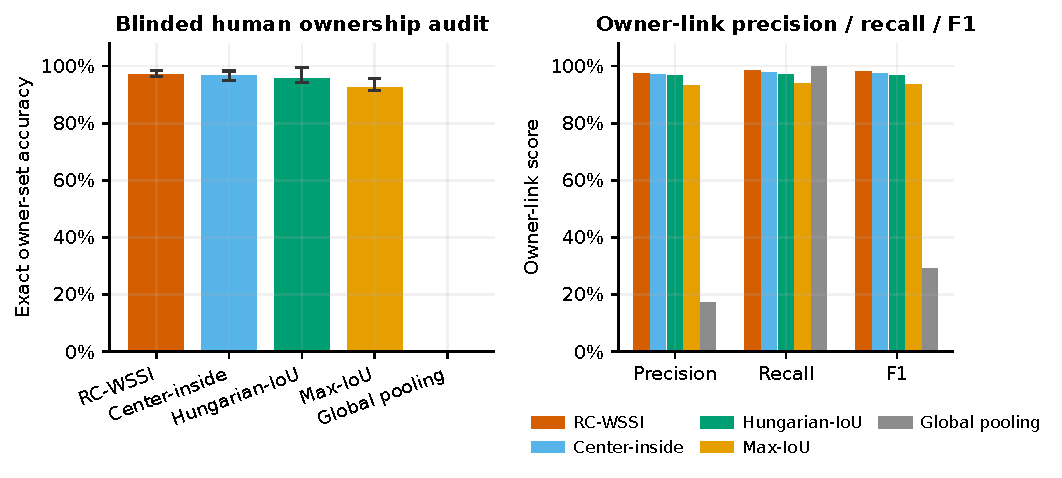
\includegraphics[width=\textwidth]{figures/v23/fig7_human_reference_assignment_audit.pdf}
\caption{Blinded, independently adjudicated human-reference audit on the selected candidate-restricted subset. Left: exact owner-set accuracy over 597 PPE boxes; whiskers are descriptive filename-group resampling intervals. Right: owner-link precision, recall, and F1. Global pooling attains link recall one by assigning each PPE box to every person, but its precision is 0.171 and it creates 2,864 extra owner links. These results concern the selected multi-worker audit subset, not full-corpus worker-state or deployment validity.}
\label{fig:humanaudit}
\end{figure*}

RC-WSSI differs from center-inside by $0.003$ in box accuracy, with paired descriptive filename-group resampling interval $[-0.005,0.019]$, and from Hungarian-IoU by $0.012$ with interval $[-0.013,0.029]$. These intervals overlap zero and do not support universal superiority over the two strong local alternatives. The difference from Max-IoU is $0.044$ with interval $[0.019,0.061]$. Class-specific RC-WSSI accuracies are 0.956 for helmet, 1.000 for no-helmet, 0.987 for reflective vest, and 1.000 for no-vest evidence. Only eight human labels are \texttt{NONE}; RC-WSSI correctly leaves two unowned, so the audit primarily supports person-owner assignment rather than unowned-object rejection.

The human audit changes the evidential boundary in one precise way: it shows that deterministic local allocation agrees with the adjudicated ownership judgments from blinded annotation on this deliberately difficult, candidate-restricted multi-worker subset. It does not convert the full filename-grouped worker-state experiments into human-semantic evaluation, because their reference states remain geometry-defined and the audit does not evaluate detector misses or temporal deployment behavior.

\subsection{Open-candidate random human-reference results}

The complementary audit evaluates the pre-frozen source-stratified random sample with a different protocol: all visible persons could be selected by each of three blind experts. Of 334 PPE rows, 13 are \texttt{AMBIGUOUS} under the predeclared three-pass rule and are excluded from exact-owner scoring; no majority label is \texttt{NONE}. Table~\ref{tab:randomaudit} therefore reports 321 determinate human-owner rows from 66 images across all 11 filename groups. The original geometric candidate set contains 320 of these 321 human owners, so the candidate restriction in the difficult audit is empirically checked on this sampled complement rather than assumed. RC-WSSI makes one owner error (320/321), while center-inside, Hungarian-IoU, and Max-IoU make 4, 2, and 3 errors. These small sampled differences are descriptive: they do not establish universal superiority of the lexicographic score. In contrast, global pooling exactly matches only 31/321 owner sets and creates 1,034 extra owner links.

\begin{table*}[t]
\caption{Open-candidate, source-stratified random human ownership audit. The 66 pre-frozen images contain 334 PPE boxes from all 11 filename groups. Thirteen three-pass \texttt{AMBIGUOUS} rows are excluded before scoring, leaving 321 determinate owner rows. Exact requires equality of the predicted and blind-majority human owner sets. Brackets are descriptive filename-group resampling intervals, not cluster-valid confidence intervals.}
\label{tab:randomaudit}
\centering
\scriptsize
\setlength{\tabcolsep}{4pt}
\resizebox{\textwidth}{!}{%
\begin{tabular}{@{}l c c c c c c@{}}
\toprule
Method & Exact & Exact accuracy [group resampling] & Image macro & Group macro & Link P/R/F1 & Extra links \\
\midrule
RC-WSSI lexicographic & 320/321 & 0.997 [0.990, 1.000] & 0.998 & 0.997 & 1.000/0.997/0.998 & 0 \\
Center-inside & 317/321 & 0.988 [0.977, 0.997] & 0.990 & 0.987 & 0.994/0.988/0.991 & 2 \\
Hungarian-IoU & 319/321 & 0.994 [0.984, 1.000] & 0.995 & 0.993 & 0.997/0.994/0.995 & 1 \\
Max-IoU & 318/321 & 0.991 [0.981, 1.000] & 0.993 & 0.991 & 0.994/0.991/0.992 & 2 \\
Global pooling & 31/321 & 0.097 [0.071, 0.128] & 0.231 & 0.103 & 0.237/1.000/0.383 & 1,034 \\
\bottomrule
\end{tabular}}
\end{table*}

The paired descriptive filename-group resampling differences for RC-WSSI are $0.009$ versus center-inside, $0.003$ versus Hungarian-IoU, and $0.006$ versus Max-IoU; all are small and are not treated as cluster-valid comparative inference. The corresponding difference from global pooling is $0.900$ (descriptive range $[0.870,0.926]$). Thus the random audit corroborates the narrower mechanism claim: single-owner allocation avoids all-to-all evidence copying and agrees closely with the sampled open-candidate human ownership reference, while the evidence does not establish RC-WSSI as a universally superior local matcher.

\subsection{Geometry-defined rule sensitivity}

We re-evaluate the frozen caches while changing one operational parameter at a time and repeating calibration. At 10\%, changing person expansion from $1.00$ to $1.30$ keeps F1 in $[0.725,0.731]$, the all-reference automatic-safe diagnostic in $[0.110,0.112]$, and composite risk in $[0.170,0.172]$. Tightening the person-match IoU from $0.40$ to $0.60$ raises the unmatched-unsafe rate from $0.051$ to $0.086$ and composite risk from $0.164$ to $0.194$, even though the all-reference automatic-safe diagnostic changes from $0.112$ to $0.108$. Raising the prediction score floor from $0.05$ to $0.20$ similarly lowers that diagnostic from $0.112$ to $0.098$ but increases unmatched unsafe persons from $0.060$ to $0.078$ and composite risk from $0.172$ to $0.176$. Replacing confidence-greedy evaluation matching by maximum-total-IoU Hungarian matching gives, at 10\%, F1/risk/composite $0.727/0.111/0.172$ versus $0.727/0.112/0.172$ for the greedy matcher; 5\% changes are similarly below 0.002. This sensitivity confirms that conditional decision risk and end-to-end composite risk answer different questions. It is a robustness analysis of the geometry-defined operational convention, not independent validation of PPE-to-worker semantic relations.

\begin{figure*}[t]
\centering
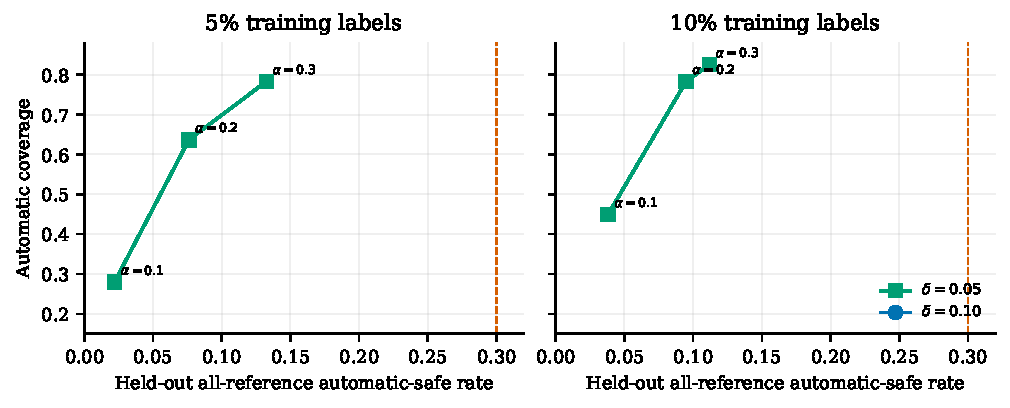
\includegraphics[width=\textwidth]{figures/v23/fig2_risk_coverage.pdf}
\caption{Held-out all-reference automatic-safe rate versus matched-person coverage from the filename-grouped sensitivity analysis. Each point is selected using calibration data only; labels show $\alpha$, and marker shape distinguishes $\delta$. The vertical line marks the feasibility setting $\alpha=0.30$.}
\label{fig:riskcoverage}
\end{figure*}

\subsection{Worker conditioning prevents global evidence sharing}

The final assignment comparison isolates the effect of allocating evidence before applying the risk rule. At 10\%, RC-WSSI obtains unsafe F1 $0.727$, automatic-safe rate $0.112$, composite rate $0.172$, and coverage $0.825$, whereas the calibrated global-pooling policy has unsafe F1 $0.280$, coverage $0.450$, and 8/15 review-all outcomes. The pooled representation allows evidence from one worker to alter every other worker's state. The fixed-threshold comparison in Table~\ref{tab:fixed_assignment} confirms that this contrast is not solely caused by calibration: pooling has high automatic coverage but much higher common-denominator automatic-safe and composite diagnostics. At the fixed threshold, paired seed--fold differences between RC-WSSI and the local rules are within $0.005$ in unsafe F1 on average; this supports the narrower claim that single-owner conditioning prevents global evidence sharing, while the particular lexicographic score is a reproducible operating rule rather than a universally optimal matcher.

The same conclusion holds at 5\%. Global pooling has unsafe F1 $0.215$ and nine review-all fallbacks, while local rules have F1 between $0.671$ and $0.683$ and no fallbacks at the primary operating point. The full-corpus worker-state comparisons in this subsection still use the same geometry-defined reference. The separate human audit in Table~\ref{tab:humanaudit} provides semantic owner evidence on 60 selected multi-worker images: it confirms high agreement for all local rules, rejects all-to-all pooling as an exact owner representation, and does not establish universal superiority of the lexicographic score.

\subsection{Real qualitative behavior}

\begin{figure*}[t]
\centering
\includegraphics[width=\textwidth]{figures/v23/fig5_real_qualitative.pdf}
\caption{Illustrative evaluation-side examples, cropped from original frames for legibility and manually privacy-redacted before rendering. Person boxes are colored by the RC-WSSI state; thin boxes and lines show the highest-confidence assigned PPE evidence per class. Labels give the geometry-defined reference (REF), RC-WSSI (RC), and, where different, global pooling (Pool), with S/U/R denoting safe/unsafe/review. (a) Missing-vest evidence makes the worker unsafe. (b) Worker allocation separates one unsafe worker from two safe workers. (c) Shared safe evidence makes global pooling accept two unsafe workers as safe, whereas RC-WSSI retains the unsafe states. (d) Weak helmet evidence leaves the worker in review rather than accepting safety. These panels illustrate the decision mechanism only; they do not replace the selected candidate-restricted human ownership audit or validate full-corpus PPE-to-worker identity.}
\label{fig:qualitative}
\end{figure*}

Figure~\ref{fig:qualitative} makes both directions of cross-worker contamination visible. Panel (b) shows how allocation preserves mixed worker states, while panel (c) shows the safety-critical failure direction quantified by the full filename-group-disjoint assignment comparison. The review example clarifies that abstention is triggered component-wise: positive vest evidence alone cannot establish safety when helmet evidence remains below threshold. Review is therefore a decision channel, not a missing binary label.

\subsection{Calibration feasibility boundary}

\begin{figure}[t]
\centering
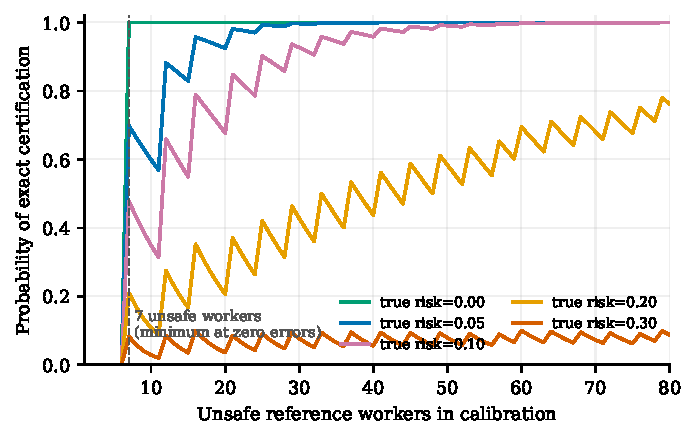
\includegraphics[width=\linewidth]{figures/v23/fig3_calibration_feasibility.pdf}
\caption{Model-conditional Clopper--Pearson retention probability as a function of all-reference unsafe calibration count and true automatic-safe rate for $\alpha=0.30$ and $\delta=0.10$. The vertical line marks the smallest count that could retain the target with zero observed errors under the independent-binomial model.}
\label{fig:feasibility}
\end{figure}

With zero observed errors, Eq.~\eqref{eq:cp} reduces to

\begin{equation}
U(0,n,\delta)=1-\delta^{1/n}.
\end{equation}

Under the independent-binomial model, retention is possible only if $n\geq\lceil\log(\delta)/\log(1-\alpha)\rceil$. For $\alpha=0.30$ and $\delta=0.10$, at least seven unsafe reference persons are needed even with zero errors. In the final filename-grouped analysis, the primary 10\% setting has no review-all fallback, whereas the stricter $\alpha=0.10$ sensitivity has 4/15 fallbacks; at 5\%, the corresponding counts are 0/15 and 8/15. Figure~\ref{fig:feasibility} separates model-based sample-size feasibility from detector accuracy and explains why a method that always emits a threshold would overstate the available evidence.

\subsection{Risk-scope sensitivity}

The three reported scopes deliberately separate selection, decision-layer behavior, and end-to-end failure. At the primary operating point, all-reference automatic-safe rate is $0.112$ at 10\% and $0.136$ at 5\%; matched-only automatic-safe rate is $0.118$ and $0.145$; composite miss-or-safe rate is $0.172$ and $0.205$. The corresponding unsafe unmatched rates are $0.060$ and $0.069$. Thus a detector miss contributes zero to the calibration event but remains in its denominator, and it is a safety error in the composite diagnostic. The full $\alpha$--$\delta$ grid, safe/unsafe/review counts, per-cell denominators, error counts, and fallback states are included in the reproducibility artifact.

\section{Discussion}\label{sec:discussion}

The main practical result is not a large F1 gain. At 10\%, the proposed rule remains close to alternative local geometric allocation rules, while global pooling produces much higher common-threshold contamination diagnostics and frequent review-all outcomes after calibration. The blinded, independently adjudicated audit sharpens this message: RC-WSSI, center-inside, and Hungarian-IoU all exceed 0.96 exact owner-set accuracy, and the paired descriptive intervals do not separate RC-WSSI from the latter two. Global pooling instead creates 2,864 extra owner links and no exact owner sets. Single-owner conditioning is therefore supported both as a contamination-control mechanism and as a high-agreement ownership representation on the audited subset, without implying that the lexicographic matcher is universally best.

The fixed-sequence calculation contributes transparent feasibility reporting. Under its worker-level Bernoulli model, its high-to-low retained prefix is selection-equivalent to a full-grid ordinary CP scan, so it is not presented as a stronger calibration method. The sensitivity analysis shows that stricter targets can force review-all: at $\alpha=0.05$, 10/15 cells at 10\% labels and 13/15 at 5\% labels return review-all. The review-all outcome distinguishes an infeasible model-conditional calculation from a retained operating point. The declared filename grouping does not establish the independence assumption needed to turn this construction into a deployment guarantee.

The threshold diagnostic is intentionally narrow and is not an end-to-end safety risk target. It is automatic safety acceptance among all unsafe geometry-defined reference persons; an unmatched unsafe person remains in this denominator but is not an automatic-safe error. The composite miss-or-safe quantity is therefore a held-out diagnostic, not a constrained quantity, and its conservative 10\% value of $0.305$ is not evidence that the $\alpha=0.30$ model-conditional diagnostic has been violated, because the composite event was not the selected event. A deployment system would require a separately specified and independently validated composite target, together with controls for person-detection recall, camera failure, temporal persistence, and human review capacity.

\section{Limitations}\label{sec:limitations}

First, the blinded, independently adjudicated difficult audit is candidate-restricted and contains 60 deliberately difficult multi-worker images selected from one corpus; its completed results establish semantic PPE ownership agreement only on that subset. The complementary source-stratified random audit is open-candidate and covers 66 images across all 11 filename groups, but it is still a finite sampled subset from the same corpus. Its three blind passes produce 13 \texttt{AMBIGUOUS} rows excluded from exact-owner scoring, and it does not establish full-corpus worker-state truth, unbiased scene prevalence, detector correctness, or temporal identity. The random audit does quantify the difficult audit's candidate restriction: 320/321 determinate random human owners fall in the original geometric candidate set, but this is sampled evidence rather than proof of universal candidate coverage. Second, experiments use one tunnel PPE corpus and two Ultralytics detector variants. The YOLO11s rerun is detector-variant robustness, not external-dataset or independent-collection validation. Third, identifiers are inferred from filenames rather than verified video, camera, date, or worker-track metadata. Repeated seed cells reuse the same filename groups, so cell and group-resampling summaries are descriptive rather than independent deployment inference. Fourth, the fixed-sequence proposition requires an independent-binomial worker-level model that the filename grouping does not establish; two calibration groups per cell are insufficient for a cluster-valid guarantee. Fifth, the 5\% and 10\% detector-training budgets use different sampled pools and are not a paired learning curve. Finally, $\alpha=0.30$ is a feasibility setting rather than an acceptable universal safety target. Deployment would require a separately calibrated composite target, verified independent clusters, external validation, and a quantified human-review process.

\section{Conclusion}\label{sec:conclusion}

RC-WSSI converts PPE detections into a deterministic single-owner representation before producing safe, unsafe, or review states. The full filename-grouped experiments show why this representation matters: all-to-all pooling shares foreign evidence, while local allocation rules behave similarly under common thresholds. The difficult audit supplies a selected candidate-restricted semantic ownership check: two experts have 587/597 row-wise exact agreements (98.32\%), a third expert resolves 10 disagreements, and RC-WSSI attains 0.975 exact owner-set accuracy on 597 boxes. The complementary open-candidate random audit supplies 321 determinate human-owner rows from 66 pre-frozen images: RC-WSSI attains 320/321 exact owner sets, and the original geometric candidate set covers 320/321 human owners. The descriptive paired group-resampling analysis shows only small differences among local rules and is not cluster-valid comparative inference, so the contribution is the single-owner representation and auditable protocol rather than a claim of universally superior matching. Global pooling is a mechanism-isolation baseline: on the random audit it matches 31/321 owner sets and its link recall of one is purchased with 1,034 extra owner links.

The threshold calculation remains a separate, narrow model-conditional diagnostic. $R_{\mathrm{auto}}$ measures a geometry-defined unsafe reference person automatically accepted as safe; the composite miss-or-safe event is not calibrated or guaranteed. The conservative reference-review-as-unsafe composite is $0.305$, compared with the default cell mean $0.172$, person-weighted $0.184$, filename-group-macro $0.243$, and observed worst filename-group/fold $0.486$. At $\alpha=0.05$, only 2/15 and 5/15 cells retain a threshold at 5\% and 10\% labels. The supported result is therefore a single-owner evidence representation assessed by a blinded, independently adjudicated audit, together with cross-worker contamination analysis and transparent selective-decision reporting, not a cluster-valid statistical or deployment safety guarantee.

\backmatter

\bmhead{Acknowledgements}
The authors acknowledge the staff responsible for collecting and managing the self-collected tunnel PPE image data and the Ultralytics open-source software ecosystem used in the experiments.

\bmhead{Statements and Declarations}

\textbf{Funding.} No external funding was received for this study.

\textbf{Competing interests.} The authors declare that they have no competing interests.

\textbf{Author contributions.} Yuge Lu: conceptualization, methodology, software, formal analysis, visualization, and original manuscript preparation. Sheng Huang, Qiuzu Lan, and Yong Cai: investigation, domain review, and manuscript review. All authors approved the final manuscript and accept responsibility for the reported work.

\textbf{Data availability.} The experiments use a self-collected low-light tunnel PPE image dataset held locally by the authoring organization. Original images, per-image annotations, detector weights, and prediction caches are not publicly available because raw construction-scene frames may contain identifiable people and are subject to organizational confidentiality and privacy controls. The public repository contains code, manuscript source, aggregate results, non-image protocol manifests, and blank annotation templates only. The corresponding author may be contacted about the feasibility of editorial data-access requests; any such access remains subject to the data owner's written authorization and applicable privacy controls and is not a promise of public or unrestricted release.

\textbf{Code availability.} The experiment and analysis scripts, manuscript source, blank human-audit templates, environment specification, and derived non-image manifests are publicly available at \url{https://github.com/eew221/11222}. The repository deliberately excludes original frames, image-derived overlays, weights, caches, and per-image labels. Before submission, the authors must create and cite a tagged immutable release of that repository and archive it with Zenodo (or an equivalent service); the resulting release identifier, commit hash, and DOI must be inserted here. This manuscript does not claim a DOI before that archival release exists.

\textbf{Ethics and privacy.} The self-collected frames may contain identifiable people. Each qualitative source crop used in Figure~\ref{fig:qualitative} was manually reviewed, and faces, badges or names, vehicle plates, company marks, and other identifiable information were strongly pixelated where present. The four-panel redaction manifest was frozen before final rendering; neither unredacted frames nor redaction overlays are released in the public repository. The authors will retain the data owner's written authorization, approval, or documented exemption basis for research use and publication of the redacted crops before submission.

\textbf{Use of AI-assisted tools.} An AI-assisted coding and language tool was used to help organize experiment code, execute reproducible analyses, and edit manuscript text. The authors verified the code, numerical claims, and references and take full responsibility for the final manuscript.

\bibliography{references}

\end{document}
